\documentclass[twoside]{book}

% Packages required by doxygen
\usepackage{fixltx2e}
\usepackage{calc}
\usepackage{doxygen}
\usepackage{graphicx}
\usepackage[utf8]{inputenc}
\usepackage{makeidx}
\usepackage{multicol}
\usepackage{multirow}
\PassOptionsToPackage{warn}{textcomp}
\usepackage{textcomp}
\usepackage[nointegrals]{wasysym}
\usepackage[table]{xcolor}

% Font selection
\usepackage[T1]{fontenc}
\usepackage{mathptmx}
\usepackage[scaled=.90]{helvet}
\usepackage{courier}
\usepackage{amssymb}
\usepackage{sectsty}
\renewcommand{\familydefault}{\sfdefault}
\allsectionsfont{%
  \fontseries{bc}\selectfont%
  \color{darkgray}%
}
\renewcommand{\DoxyLabelFont}{%
  \fontseries{bc}\selectfont%
  \color{darkgray}%
}
\newcommand{\+}{\discretionary{\mbox{\scriptsize$\hookleftarrow$}}{}{}}

% Page & text layout
\usepackage{geometry}
\geometry{%
  a4paper,%
  top=2.5cm,%
  bottom=2.5cm,%
  left=2.5cm,%
  right=2.5cm%
}
\tolerance=750
\hfuzz=15pt
\hbadness=750
\setlength{\emergencystretch}{15pt}
\setlength{\parindent}{0cm}
\setlength{\parskip}{0.2cm}
\makeatletter
\renewcommand{\paragraph}{%
  \@startsection{paragraph}{4}{0ex}{-1.0ex}{1.0ex}{%
    \normalfont\normalsize\bfseries\SS@parafont%
  }%
}
\renewcommand{\subparagraph}{%
  \@startsection{subparagraph}{5}{0ex}{-1.0ex}{1.0ex}{%
    \normalfont\normalsize\bfseries\SS@subparafont%
  }%
}
\makeatother

% Headers & footers
\usepackage{fancyhdr}
\pagestyle{fancyplain}
\fancyhead[LE]{\fancyplain{}{\bfseries\thepage}}
\fancyhead[CE]{\fancyplain{}{}}
\fancyhead[RE]{\fancyplain{}{\bfseries\leftmark}}
\fancyhead[LO]{\fancyplain{}{\bfseries\rightmark}}
\fancyhead[CO]{\fancyplain{}{}}
\fancyhead[RO]{\fancyplain{}{\bfseries\thepage}}
\fancyfoot[LE]{\fancyplain{}{}}
\fancyfoot[CE]{\fancyplain{}{}}
\fancyfoot[RE]{\fancyplain{}{\bfseries\scriptsize Generated on Wed Nov 5 2014 20\+:22\+:57 for Rescue A by Doxygen }}
\fancyfoot[LO]{\fancyplain{}{\bfseries\scriptsize Generated on Wed Nov 5 2014 20\+:22\+:57 for Rescue A by Doxygen }}
\fancyfoot[CO]{\fancyplain{}{}}
\fancyfoot[RO]{\fancyplain{}{}}
\renewcommand{\footrulewidth}{0.4pt}
\renewcommand{\chaptermark}[1]{%
  \markboth{#1}{}%
}
\renewcommand{\sectionmark}[1]{%
  \markright{\thesection\ #1}%
}

% Indices & bibliography
\usepackage{natbib}
\usepackage[titles]{tocloft}
\setcounter{tocdepth}{3}
\setcounter{secnumdepth}{5}
\makeindex

% Hyperlinks (required, but should be loaded last)
\usepackage{ifpdf}
\ifpdf
  \usepackage[pdftex,pagebackref=true]{hyperref}
\else
  \usepackage[ps2pdf,pagebackref=true]{hyperref}
\fi
\hypersetup{%
  colorlinks=true,%
  linkcolor=blue,%
  citecolor=blue,%
  unicode%
}

% Custom commands
\newcommand{\clearemptydoublepage}{%
  \newpage{\pagestyle{empty}\cleardoublepage}%
}


%===== C O N T E N T S =====

\begin{document}

% Titlepage & ToC
\hypersetup{pageanchor=false,
             bookmarks=true,
             bookmarksnumbered=true,
             pdfencoding=unicode
            }
\pagenumbering{roman}
\begin{titlepage}
\vspace*{7cm}
\begin{center}%
{\Large Rescue A }\\
\vspace*{1cm}
{\large Generated by Doxygen 1.8.8}\\
\vspace*{0.5cm}
{\small Wed Nov 5 2014 20:22:57}\\
\end{center}
\end{titlepage}
\clearemptydoublepage
\tableofcontents
\clearemptydoublepage
\pagenumbering{arabic}
\hypersetup{pageanchor=true}

%--- Begin generated contents ---
\chapter{Hierarchical Index}
\section{Class Hierarchy}
This inheritance list is sorted roughly, but not completely, alphabetically\+:\begin{DoxyCompactList}
\item Callback\begin{DoxyCompactList}
\item \contentsline{section}{com.\+aronbordin.\+robo.\+camera.\+Camera\+Robo}{\pageref{d6/dc1/classcom_1_1aronbordin_1_1robo_1_1camera_1_1CameraRobo}}{}
\end{DoxyCompactList}
\item \contentsline{section}{com.\+aronbordin.\+robo.\+camera.\+Logger}{\pageref{d4/d13/classcom_1_1aronbordin_1_1robo_1_1camera_1_1Logger}}{}
\item On\+Touch\+Listener\begin{DoxyCompactList}
\item \contentsline{section}{com.\+aronbordin.\+robo.\+camera.\+Camera\+Robo}{\pageref{d6/dc1/classcom_1_1aronbordin_1_1robo_1_1camera_1_1CameraRobo}}{}
\end{DoxyCompactList}
\item Preview\+Callback\begin{DoxyCompactList}
\item \contentsline{section}{com.\+aronbordin.\+robo.\+camera.\+Camera\+Robo}{\pageref{d6/dc1/classcom_1_1aronbordin_1_1robo_1_1camera_1_1CameraRobo}}{}
\end{DoxyCompactList}
\item Thread\begin{DoxyCompactList}
\item \contentsline{section}{com.\+aronbordin.\+robo.\+camera.\+Bluetooth\+Robo}{\pageref{da/df5/classcom_1_1aronbordin_1_1robo_1_1camera_1_1BluetoothRobo}}{}
\item \contentsline{section}{com.\+aronbordin.\+robo.\+camera.\+Robo}{\pageref{df/d6a/classcom_1_1aronbordin_1_1robo_1_1camera_1_1Robo}}{}
\end{DoxyCompactList}
\item Activity\begin{DoxyCompactList}
\item \contentsline{section}{com.\+aronbordin.\+robo.\+camera.\+Main\+Activity}{\pageref{dd/da1/classcom_1_1aronbordin_1_1robo_1_1camera_1_1MainActivity}}{}
\end{DoxyCompactList}
\item Surface\+View\begin{DoxyCompactList}
\item \contentsline{section}{com.\+aronbordin.\+robo.\+camera.\+Camera\+Robo}{\pageref{d6/dc1/classcom_1_1aronbordin_1_1robo_1_1camera_1_1CameraRobo}}{}
\end{DoxyCompactList}
\end{DoxyCompactList}

\chapter{Class Index}
\section{Class List}
Here are the classes, structs, unions and interfaces with brief descriptions\+:\begin{DoxyCompactList}
\item\contentsline{section}{\hyperlink{classcom_1_1aronbordin_1_1robo_1_1camera_1_1BluetoothRobo}{com.\+aronbordin.\+robo.\+camera.\+Bluetooth\+Robo} }{\pageref{da/df5/classcom_1_1aronbordin_1_1robo_1_1camera_1_1BluetoothRobo}}{}
\item\contentsline{section}{\hyperlink{classcom_1_1aronbordin_1_1robo_1_1camera_1_1CameraRobo}{com.\+aronbordin.\+robo.\+camera.\+Camera\+Robo} }{\pageref{d6/dc1/classcom_1_1aronbordin_1_1robo_1_1camera_1_1CameraRobo}}{}
\item\contentsline{section}{\hyperlink{classcom_1_1aronbordin_1_1robo_1_1camera_1_1Logger}{com.\+aronbordin.\+robo.\+camera.\+Logger} }{\pageref{d4/d13/classcom_1_1aronbordin_1_1robo_1_1camera_1_1Logger}}{}
\item\contentsline{section}{\hyperlink{classcom_1_1aronbordin_1_1robo_1_1camera_1_1MainActivity}{com.\+aronbordin.\+robo.\+camera.\+Main\+Activity} }{\pageref{dd/da1/classcom_1_1aronbordin_1_1robo_1_1camera_1_1MainActivity}}{}
\item\contentsline{section}{\hyperlink{classcom_1_1aronbordin_1_1robo_1_1camera_1_1Robo}{com.\+aronbordin.\+robo.\+camera.\+Robo} }{\pageref{df/d6a/classcom_1_1aronbordin_1_1robo_1_1camera_1_1Robo}}{}
\end{DoxyCompactList}

\chapter{Class Documentation}
\hypertarget{classcom_1_1aronbordin_1_1robo_1_1camera_1_1BluetoothRobo}{\section{com.\+aronbordin.\+robo.\+camera.\+Bluetooth\+Robo Class Reference}
\label{classcom_1_1aronbordin_1_1robo_1_1camera_1_1BluetoothRobo}\index{com.\+aronbordin.\+robo.\+camera.\+Bluetooth\+Robo@{com.\+aronbordin.\+robo.\+camera.\+Bluetooth\+Robo}}
}
Inheritance diagram for com.\+aronbordin.\+robo.\+camera.\+Bluetooth\+Robo\+:\begin{figure}[H]
\begin{center}
\leavevmode
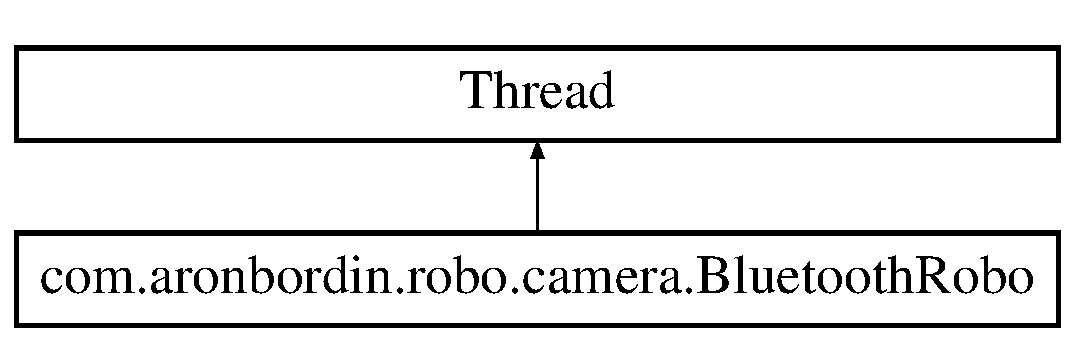
\includegraphics[height=2.000000cm]{da/df5/classcom_1_1aronbordin_1_1robo_1_1camera_1_1BluetoothRobo}
\end{center}
\end{figure}
\subsection*{Public Member Functions}
\begin{DoxyCompactItemize}
\item 
\hypertarget{classcom_1_1aronbordin_1_1robo_1_1camera_1_1BluetoothRobo_a27e09a097a737dfe4fefea2299410ece}{boolean {\bfseries conectado} ()}\label{classcom_1_1aronbordin_1_1robo_1_1camera_1_1BluetoothRobo_a27e09a097a737dfe4fefea2299410ece}

\item 
void \hyperlink{classcom_1_1aronbordin_1_1robo_1_1camera_1_1BluetoothRobo_a2df2abd3a673b28ce8c15485bbfa7445}{Conectar} ()
\item 
void \hyperlink{classcom_1_1aronbordin_1_1robo_1_1camera_1_1BluetoothRobo_a91456e33e64f7b6014eec4aab7e2aa41}{run} ()
\item 
boolean \hyperlink{classcom_1_1aronbordin_1_1robo_1_1camera_1_1BluetoothRobo_a6f90297b6ea2088d8386ef9903e8f879}{has\+Mensagem} (int i)
\item 
String \hyperlink{classcom_1_1aronbordin_1_1robo_1_1camera_1_1BluetoothRobo_adec3780ecaa5fdda458c88fb7c0614dd}{get\+Mensagem} (int i)
\item 
void \hyperlink{classcom_1_1aronbordin_1_1robo_1_1camera_1_1BluetoothRobo_acc329c69c4399635133fc72f85f696be}{enviar\+Msg} (String msg)
\end{DoxyCompactItemize}


\subsection{Detailed Description}
Created by neo on 08/06/14. \begin{DoxyAuthor}{Author}
Aron Bordin \href{mailto:aron.bordin@gmail.com}{\tt aron.\+bordin@gmail.\+com} Classe para gerenciar conexão bluetooth. 
\end{DoxyAuthor}


\subsection{Member Function Documentation}
\hypertarget{classcom_1_1aronbordin_1_1robo_1_1camera_1_1BluetoothRobo_a2df2abd3a673b28ce8c15485bbfa7445}{\index{com\+::aronbordin\+::robo\+::camera\+::\+Bluetooth\+Robo@{com\+::aronbordin\+::robo\+::camera\+::\+Bluetooth\+Robo}!Conectar@{Conectar}}
\index{Conectar@{Conectar}!com\+::aronbordin\+::robo\+::camera\+::\+Bluetooth\+Robo@{com\+::aronbordin\+::robo\+::camera\+::\+Bluetooth\+Robo}}
\subsubsection[{Conectar}]{\setlength{\rightskip}{0pt plus 5cm}void com.\+aronbordin.\+robo.\+camera.\+Bluetooth\+Robo.\+Conectar (
\begin{DoxyParamCaption}
{}
\end{DoxyParamCaption}
)\hspace{0.3cm}{\ttfamily [inline]}}}\label{classcom_1_1aronbordin_1_1robo_1_1camera_1_1BluetoothRobo_a2df2abd3a673b28ce8c15485bbfa7445}
Realiza a conexão com o robo via bluetooth. Caso tenha algum problema, informa no log. \hypertarget{classcom_1_1aronbordin_1_1robo_1_1camera_1_1BluetoothRobo_acc329c69c4399635133fc72f85f696be}{\index{com\+::aronbordin\+::robo\+::camera\+::\+Bluetooth\+Robo@{com\+::aronbordin\+::robo\+::camera\+::\+Bluetooth\+Robo}!enviar\+Msg@{enviar\+Msg}}
\index{enviar\+Msg@{enviar\+Msg}!com\+::aronbordin\+::robo\+::camera\+::\+Bluetooth\+Robo@{com\+::aronbordin\+::robo\+::camera\+::\+Bluetooth\+Robo}}
\subsubsection[{enviar\+Msg}]{\setlength{\rightskip}{0pt plus 5cm}void com.\+aronbordin.\+robo.\+camera.\+Bluetooth\+Robo.\+enviar\+Msg (
\begin{DoxyParamCaption}
\item[{String}]{msg}
\end{DoxyParamCaption}
)\hspace{0.3cm}{\ttfamily [inline]}}}\label{classcom_1_1aronbordin_1_1robo_1_1camera_1_1BluetoothRobo_acc329c69c4399635133fc72f85f696be}
Método para enviar mensagem por bluetooth 
\begin{DoxyParams}{Parameters}
{\em msg} & Mensagem a ser enviada \\
\hline
\end{DoxyParams}
\hypertarget{classcom_1_1aronbordin_1_1robo_1_1camera_1_1BluetoothRobo_adec3780ecaa5fdda458c88fb7c0614dd}{\index{com\+::aronbordin\+::robo\+::camera\+::\+Bluetooth\+Robo@{com\+::aronbordin\+::robo\+::camera\+::\+Bluetooth\+Robo}!get\+Mensagem@{get\+Mensagem}}
\index{get\+Mensagem@{get\+Mensagem}!com\+::aronbordin\+::robo\+::camera\+::\+Bluetooth\+Robo@{com\+::aronbordin\+::robo\+::camera\+::\+Bluetooth\+Robo}}
\subsubsection[{get\+Mensagem}]{\setlength{\rightskip}{0pt plus 5cm}String com.\+aronbordin.\+robo.\+camera.\+Bluetooth\+Robo.\+get\+Mensagem (
\begin{DoxyParamCaption}
\item[{int}]{i}
\end{DoxyParamCaption}
)\hspace{0.3cm}{\ttfamily [inline]}}}\label{classcom_1_1aronbordin_1_1robo_1_1camera_1_1BluetoothRobo_adec3780ecaa5fdda458c88fb7c0614dd}
Retorna uma mensagem por id. Caso a mensagem não existe, será retornada uma string vazia 
\begin{DoxyParams}{Parameters}
{\em i} & I\+D da Mensagem \\
\hline
\end{DoxyParams}
\begin{DoxyReturn}{Returns}

\end{DoxyReturn}
\hypertarget{classcom_1_1aronbordin_1_1robo_1_1camera_1_1BluetoothRobo_a6f90297b6ea2088d8386ef9903e8f879}{\index{com\+::aronbordin\+::robo\+::camera\+::\+Bluetooth\+Robo@{com\+::aronbordin\+::robo\+::camera\+::\+Bluetooth\+Robo}!has\+Mensagem@{has\+Mensagem}}
\index{has\+Mensagem@{has\+Mensagem}!com\+::aronbordin\+::robo\+::camera\+::\+Bluetooth\+Robo@{com\+::aronbordin\+::robo\+::camera\+::\+Bluetooth\+Robo}}
\subsubsection[{has\+Mensagem}]{\setlength{\rightskip}{0pt plus 5cm}boolean com.\+aronbordin.\+robo.\+camera.\+Bluetooth\+Robo.\+has\+Mensagem (
\begin{DoxyParamCaption}
\item[{int}]{i}
\end{DoxyParamCaption}
)\hspace{0.3cm}{\ttfamily [inline]}}}\label{classcom_1_1aronbordin_1_1robo_1_1camera_1_1BluetoothRobo_a6f90297b6ea2088d8386ef9903e8f879}
Testa se a mensage foi recebida de acordo com o I\+D do pedido 
\begin{DoxyParams}{Parameters}
{\em i} & I\+D da Mensagem \\
\hline
\end{DoxyParams}
\begin{DoxyReturn}{Returns}
boolean, indicando se a mensagem foi recebida 
\end{DoxyReturn}
\hypertarget{classcom_1_1aronbordin_1_1robo_1_1camera_1_1BluetoothRobo_a91456e33e64f7b6014eec4aab7e2aa41}{\index{com\+::aronbordin\+::robo\+::camera\+::\+Bluetooth\+Robo@{com\+::aronbordin\+::robo\+::camera\+::\+Bluetooth\+Robo}!run@{run}}
\index{run@{run}!com\+::aronbordin\+::robo\+::camera\+::\+Bluetooth\+Robo@{com\+::aronbordin\+::robo\+::camera\+::\+Bluetooth\+Robo}}
\subsubsection[{run}]{\setlength{\rightskip}{0pt plus 5cm}void com.\+aronbordin.\+robo.\+camera.\+Bluetooth\+Robo.\+run (
\begin{DoxyParamCaption}
{}
\end{DoxyParamCaption}
)\hspace{0.3cm}{\ttfamily [inline]}}}\label{classcom_1_1aronbordin_1_1robo_1_1camera_1_1BluetoothRobo_a91456e33e64f7b6014eec4aab7e2aa41}
Inicia o Thread para ficar checando se novas mensagens chegaram. Não use essa função!! Ela será usada internamente pela classe, caso seja utilizada em outro local, não irá funcionar 

The documentation for this class was generated from the following file\+:\begin{DoxyCompactItemize}
\item 
aronbordin/robo/camera/Bluetooth\+Robo.\+java\end{DoxyCompactItemize}

\hypertarget{classcom_1_1aronbordin_1_1robo_1_1camera_1_1CameraRobo}{\section{com.\+aronbordin.\+robo.\+camera.\+Camera\+Robo Class Reference}
\label{classcom_1_1aronbordin_1_1robo_1_1camera_1_1CameraRobo}\index{com.\+aronbordin.\+robo.\+camera.\+Camera\+Robo@{com.\+aronbordin.\+robo.\+camera.\+Camera\+Robo}}
}
Inheritance diagram for com.\+aronbordin.\+robo.\+camera.\+Camera\+Robo\+:\begin{figure}[H]
\begin{center}
\leavevmode
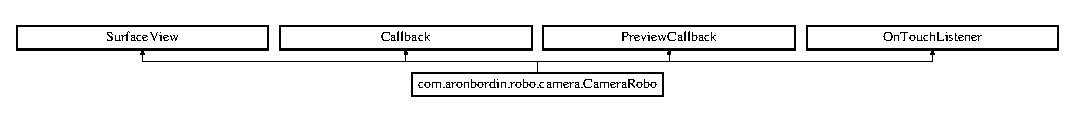
\includegraphics[height=1.068702cm]{d6/dc1/classcom_1_1aronbordin_1_1robo_1_1camera_1_1CameraRobo}
\end{center}
\end{figure}
\subsection*{Public Member Functions}
\begin{DoxyCompactItemize}
\item 
\hypertarget{classcom_1_1aronbordin_1_1robo_1_1camera_1_1CameraRobo_a2dcd4415d9acc0de33e6bed7cc843c6e}{void {\bfseries surface\+Created} (Surface\+Holder surface\+Holder)}\label{classcom_1_1aronbordin_1_1robo_1_1camera_1_1CameraRobo_a2dcd4415d9acc0de33e6bed7cc843c6e}

\item 
\hypertarget{classcom_1_1aronbordin_1_1robo_1_1camera_1_1CameraRobo_a88bfbd15922bb82b51cc33f0d401c602}{void {\bfseries surface\+Changed} (Surface\+Holder surface\+Holder, int i, int i2, int i3)}\label{classcom_1_1aronbordin_1_1robo_1_1camera_1_1CameraRobo_a88bfbd15922bb82b51cc33f0d401c602}

\item 
\hypertarget{classcom_1_1aronbordin_1_1robo_1_1camera_1_1CameraRobo_afd381329a45a7ee2ad06e47d0b917e3c}{void {\bfseries surface\+Destroyed} (Surface\+Holder surface\+Holder)}\label{classcom_1_1aronbordin_1_1robo_1_1camera_1_1CameraRobo_afd381329a45a7ee2ad06e47d0b917e3c}

\item 
void \hyperlink{classcom_1_1aronbordin_1_1robo_1_1camera_1_1CameraRobo_a0ccae659a8cdca149c700c82480a69dd}{on\+Preview\+Frame} (byte\mbox{[}$\,$\mbox{]} data, Camera camera)
\item 
void \hyperlink{classcom_1_1aronbordin_1_1robo_1_1camera_1_1CameraRobo_a90875b856ac94bf73ca48e46d2216c21}{set\+Is\+Rodando} (boolean rodando)
\item 
void \hyperlink{classcom_1_1aronbordin_1_1robo_1_1camera_1_1CameraRobo_adf16c2b85ed6dd6e9e486d3592547e86}{Processar} ()
\item 
boolean \hyperlink{classcom_1_1aronbordin_1_1robo_1_1camera_1_1CameraRobo_a84604cfcd672cac7046b0eb9e4fccf1b}{Dados\+Processados} ()
\item 
int \hyperlink{classcom_1_1aronbordin_1_1robo_1_1camera_1_1CameraRobo_aa4a9a1f4266f8706f7ce0f7db77fa1ad}{is\+Preto} (int k)
\item 
int \hyperlink{classcom_1_1aronbordin_1_1robo_1_1camera_1_1CameraRobo_ac34a9602b2ee4d84d1b3deb016b932ef}{is\+Branco} (int k)
\item 
boolean \hyperlink{classcom_1_1aronbordin_1_1robo_1_1camera_1_1CameraRobo_a290f5d43c351368627e558213a873fb3}{on\+Touch} (View v, Motion\+Event event)
\end{DoxyCompactItemize}
\subsection*{Protected Member Functions}
\begin{DoxyCompactItemize}
\item 
void \hyperlink{classcom_1_1aronbordin_1_1robo_1_1camera_1_1CameraRobo_a704dc5a516ffce7a2eac4e421469163e}{zerar\+Calibrar} ()
\item 
void \hyperlink{classcom_1_1aronbordin_1_1robo_1_1camera_1_1CameraRobo_ae0899639ec813e5e16cc88b5a105acdd}{Calibrar} ()
\item 
void \hyperlink{classcom_1_1aronbordin_1_1robo_1_1camera_1_1CameraRobo_adcbe43b99dd1a3e9ef9133ddfc890b0e}{Calibrar\+Fim} ()
\item 
\hypertarget{classcom_1_1aronbordin_1_1robo_1_1camera_1_1CameraRobo_a1ddfd5a73b58dc9330c03ffb661420cc}{void {\bfseries on\+Draw} (Canvas canvas)}\label{classcom_1_1aronbordin_1_1robo_1_1camera_1_1CameraRobo_a1ddfd5a73b58dc9330c03ffb661420cc}

\item 
void \hyperlink{classcom_1_1aronbordin_1_1robo_1_1camera_1_1CameraRobo_ac95f2722132d4dd85d7bca5b9cd9ce7b}{decode\+Y\+U\+V420\+S\+P} (int\mbox{[}$\,$\mbox{]} rgb, byte\mbox{[}$\,$\mbox{]} yuv420sp, int width, int height)
\end{DoxyCompactItemize}


\subsection{Detailed Description}
Created by neo on 06/06/14. \begin{DoxyAuthor}{Author}
Aron Bordin \href{mailto:aron.bordin@gmail.com}{\tt aron.\+bordin@gmail.\+com} Classe para gerenciar a camera do robô. Irá analisar as imagens, e contém helpers para ler seu conteúdo 
\end{DoxyAuthor}


\subsection{Member Function Documentation}
\hypertarget{classcom_1_1aronbordin_1_1robo_1_1camera_1_1CameraRobo_ae0899639ec813e5e16cc88b5a105acdd}{\index{com\+::aronbordin\+::robo\+::camera\+::\+Camera\+Robo@{com\+::aronbordin\+::robo\+::camera\+::\+Camera\+Robo}!Calibrar@{Calibrar}}
\index{Calibrar@{Calibrar}!com\+::aronbordin\+::robo\+::camera\+::\+Camera\+Robo@{com\+::aronbordin\+::robo\+::camera\+::\+Camera\+Robo}}
\subsubsection[{Calibrar}]{\setlength{\rightskip}{0pt plus 5cm}void com.\+aronbordin.\+robo.\+camera.\+Camera\+Robo.\+Calibrar (
\begin{DoxyParamCaption}
{}
\end{DoxyParamCaption}
)\hspace{0.3cm}{\ttfamily [inline]}, {\ttfamily [protected]}}}\label{classcom_1_1aronbordin_1_1robo_1_1camera_1_1CameraRobo_ae0899639ec813e5e16cc88b5a105acdd}
Calibra a camera com o ambiente \hypertarget{classcom_1_1aronbordin_1_1robo_1_1camera_1_1CameraRobo_adcbe43b99dd1a3e9ef9133ddfc890b0e}{\index{com\+::aronbordin\+::robo\+::camera\+::\+Camera\+Robo@{com\+::aronbordin\+::robo\+::camera\+::\+Camera\+Robo}!Calibrar\+Fim@{Calibrar\+Fim}}
\index{Calibrar\+Fim@{Calibrar\+Fim}!com\+::aronbordin\+::robo\+::camera\+::\+Camera\+Robo@{com\+::aronbordin\+::robo\+::camera\+::\+Camera\+Robo}}
\subsubsection[{Calibrar\+Fim}]{\setlength{\rightskip}{0pt plus 5cm}void com.\+aronbordin.\+robo.\+camera.\+Camera\+Robo.\+Calibrar\+Fim (
\begin{DoxyParamCaption}
{}
\end{DoxyParamCaption}
)\hspace{0.3cm}{\ttfamily [inline]}, {\ttfamily [protected]}}}\label{classcom_1_1aronbordin_1_1robo_1_1camera_1_1CameraRobo_adcbe43b99dd1a3e9ef9133ddfc890b0e}
Termina a calibração, analisando os dados coletados e gerando os novos limites \hypertarget{classcom_1_1aronbordin_1_1robo_1_1camera_1_1CameraRobo_a84604cfcd672cac7046b0eb9e4fccf1b}{\index{com\+::aronbordin\+::robo\+::camera\+::\+Camera\+Robo@{com\+::aronbordin\+::robo\+::camera\+::\+Camera\+Robo}!Dados\+Processados@{Dados\+Processados}}
\index{Dados\+Processados@{Dados\+Processados}!com\+::aronbordin\+::robo\+::camera\+::\+Camera\+Robo@{com\+::aronbordin\+::robo\+::camera\+::\+Camera\+Robo}}
\subsubsection[{Dados\+Processados}]{\setlength{\rightskip}{0pt plus 5cm}boolean com.\+aronbordin.\+robo.\+camera.\+Camera\+Robo.\+Dados\+Processados (
\begin{DoxyParamCaption}
{}
\end{DoxyParamCaption}
)\hspace{0.3cm}{\ttfamily [inline]}}}\label{classcom_1_1aronbordin_1_1robo_1_1camera_1_1CameraRobo_a84604cfcd672cac7046b0eb9e4fccf1b}
Informa se os dados já foram processados \begin{DoxyReturn}{Returns}
boolean se os dados já foram analisados 
\end{DoxyReturn}
\hypertarget{classcom_1_1aronbordin_1_1robo_1_1camera_1_1CameraRobo_ac95f2722132d4dd85d7bca5b9cd9ce7b}{\index{com\+::aronbordin\+::robo\+::camera\+::\+Camera\+Robo@{com\+::aronbordin\+::robo\+::camera\+::\+Camera\+Robo}!decode\+Y\+U\+V420\+S\+P@{decode\+Y\+U\+V420\+S\+P}}
\index{decode\+Y\+U\+V420\+S\+P@{decode\+Y\+U\+V420\+S\+P}!com\+::aronbordin\+::robo\+::camera\+::\+Camera\+Robo@{com\+::aronbordin\+::robo\+::camera\+::\+Camera\+Robo}}
\subsubsection[{decode\+Y\+U\+V420\+S\+P}]{\setlength{\rightskip}{0pt plus 5cm}void com.\+aronbordin.\+robo.\+camera.\+Camera\+Robo.\+decode\+Y\+U\+V420\+S\+P (
\begin{DoxyParamCaption}
\item[{int\mbox{[}$\,$\mbox{]}}]{rgb, }
\item[{byte\mbox{[}$\,$\mbox{]}}]{yuv420sp, }
\item[{int}]{width, }
\item[{int}]{height}
\end{DoxyParamCaption}
)\hspace{0.3cm}{\ttfamily [inline]}, {\ttfamily [protected]}}}\label{classcom_1_1aronbordin_1_1robo_1_1camera_1_1CameraRobo_ac95f2722132d4dd85d7bca5b9cd9ce7b}
Converte o formato da imagem 
\begin{DoxyParams}{Parameters}
{\em rgb} & \\
\hline
{\em yuv420sp} & \\
\hline
{\em width} & \\
\hline
{\em height} & \\
\hline
\end{DoxyParams}
\hypertarget{classcom_1_1aronbordin_1_1robo_1_1camera_1_1CameraRobo_ac34a9602b2ee4d84d1b3deb016b932ef}{\index{com\+::aronbordin\+::robo\+::camera\+::\+Camera\+Robo@{com\+::aronbordin\+::robo\+::camera\+::\+Camera\+Robo}!is\+Branco@{is\+Branco}}
\index{is\+Branco@{is\+Branco}!com\+::aronbordin\+::robo\+::camera\+::\+Camera\+Robo@{com\+::aronbordin\+::robo\+::camera\+::\+Camera\+Robo}}
\subsubsection[{is\+Branco}]{\setlength{\rightskip}{0pt plus 5cm}int com.\+aronbordin.\+robo.\+camera.\+Camera\+Robo.\+is\+Branco (
\begin{DoxyParamCaption}
\item[{int}]{k}
\end{DoxyParamCaption}
)\hspace{0.3cm}{\ttfamily [inline]}}}\label{classcom_1_1aronbordin_1_1robo_1_1camera_1_1CameraRobo_ac34a9602b2ee4d84d1b3deb016b932ef}
Testa se o bloco desejado é branco 
\begin{DoxyParams}{Parameters}
{\em k} & I\+D do bloco, de 0 à 4 \\
\hline
\end{DoxyParams}
\begin{DoxyReturn}{Returns}
1 se igual a branco, 0 se preto 
\end{DoxyReturn}
\hypertarget{classcom_1_1aronbordin_1_1robo_1_1camera_1_1CameraRobo_aa4a9a1f4266f8706f7ce0f7db77fa1ad}{\index{com\+::aronbordin\+::robo\+::camera\+::\+Camera\+Robo@{com\+::aronbordin\+::robo\+::camera\+::\+Camera\+Robo}!is\+Preto@{is\+Preto}}
\index{is\+Preto@{is\+Preto}!com\+::aronbordin\+::robo\+::camera\+::\+Camera\+Robo@{com\+::aronbordin\+::robo\+::camera\+::\+Camera\+Robo}}
\subsubsection[{is\+Preto}]{\setlength{\rightskip}{0pt plus 5cm}int com.\+aronbordin.\+robo.\+camera.\+Camera\+Robo.\+is\+Preto (
\begin{DoxyParamCaption}
\item[{int}]{k}
\end{DoxyParamCaption}
)\hspace{0.3cm}{\ttfamily [inline]}}}\label{classcom_1_1aronbordin_1_1robo_1_1camera_1_1CameraRobo_aa4a9a1f4266f8706f7ce0f7db77fa1ad}
Testa se o bloco desejado é preto 
\begin{DoxyParams}{Parameters}
{\em k} & I\+D do bloco, de 0 à 4 \\
\hline
\end{DoxyParams}
\begin{DoxyReturn}{Returns}
1 se igual a preto, 0 se branco 
\end{DoxyReturn}
\hypertarget{classcom_1_1aronbordin_1_1robo_1_1camera_1_1CameraRobo_a0ccae659a8cdca149c700c82480a69dd}{\index{com\+::aronbordin\+::robo\+::camera\+::\+Camera\+Robo@{com\+::aronbordin\+::robo\+::camera\+::\+Camera\+Robo}!on\+Preview\+Frame@{on\+Preview\+Frame}}
\index{on\+Preview\+Frame@{on\+Preview\+Frame}!com\+::aronbordin\+::robo\+::camera\+::\+Camera\+Robo@{com\+::aronbordin\+::robo\+::camera\+::\+Camera\+Robo}}
\subsubsection[{on\+Preview\+Frame}]{\setlength{\rightskip}{0pt plus 5cm}void com.\+aronbordin.\+robo.\+camera.\+Camera\+Robo.\+on\+Preview\+Frame (
\begin{DoxyParamCaption}
\item[{byte\mbox{[}$\,$\mbox{]}}]{data, }
\item[{Camera}]{camera}
\end{DoxyParamCaption}
)\hspace{0.3cm}{\ttfamily [inline]}}}\label{classcom_1_1aronbordin_1_1robo_1_1camera_1_1CameraRobo_a0ccae659a8cdca149c700c82480a69dd}
Callback chamado a cada novo frame da camera 
\begin{DoxyParams}{Parameters}
{\em data} & array de bytes, onde cada byte representa um pixel \\
\hline
{\em camera} & objeto camera \\
\hline
\end{DoxyParams}
\hypertarget{classcom_1_1aronbordin_1_1robo_1_1camera_1_1CameraRobo_a290f5d43c351368627e558213a873fb3}{\index{com\+::aronbordin\+::robo\+::camera\+::\+Camera\+Robo@{com\+::aronbordin\+::robo\+::camera\+::\+Camera\+Robo}!on\+Touch@{on\+Touch}}
\index{on\+Touch@{on\+Touch}!com\+::aronbordin\+::robo\+::camera\+::\+Camera\+Robo@{com\+::aronbordin\+::robo\+::camera\+::\+Camera\+Robo}}
\subsubsection[{on\+Touch}]{\setlength{\rightskip}{0pt plus 5cm}boolean com.\+aronbordin.\+robo.\+camera.\+Camera\+Robo.\+on\+Touch (
\begin{DoxyParamCaption}
\item[{View}]{v, }
\item[{Motion\+Event}]{event}
\end{DoxyParamCaption}
)\hspace{0.3cm}{\ttfamily [inline]}}}\label{classcom_1_1aronbordin_1_1robo_1_1camera_1_1CameraRobo_a290f5d43c351368627e558213a873fb3}
Gerencia os toques na tela 
\begin{DoxyParams}{Parameters}
{\em v} & Vie \\
\hline
{\em event} & Evnto \\
\hline
\end{DoxyParams}
\begin{DoxyReturn}{Returns}
True se o evento foi analisado 
\end{DoxyReturn}
\hypertarget{classcom_1_1aronbordin_1_1robo_1_1camera_1_1CameraRobo_adf16c2b85ed6dd6e9e486d3592547e86}{\index{com\+::aronbordin\+::robo\+::camera\+::\+Camera\+Robo@{com\+::aronbordin\+::robo\+::camera\+::\+Camera\+Robo}!Processar@{Processar}}
\index{Processar@{Processar}!com\+::aronbordin\+::robo\+::camera\+::\+Camera\+Robo@{com\+::aronbordin\+::robo\+::camera\+::\+Camera\+Robo}}
\subsubsection[{Processar}]{\setlength{\rightskip}{0pt plus 5cm}void com.\+aronbordin.\+robo.\+camera.\+Camera\+Robo.\+Processar (
\begin{DoxyParamCaption}
{}
\end{DoxyParamCaption}
)\hspace{0.3cm}{\ttfamily [inline]}}}\label{classcom_1_1aronbordin_1_1robo_1_1camera_1_1CameraRobo_adf16c2b85ed6dd6e9e486d3592547e86}
Permite o processamento de imagens \hypertarget{classcom_1_1aronbordin_1_1robo_1_1camera_1_1CameraRobo_a90875b856ac94bf73ca48e46d2216c21}{\index{com\+::aronbordin\+::robo\+::camera\+::\+Camera\+Robo@{com\+::aronbordin\+::robo\+::camera\+::\+Camera\+Robo}!set\+Is\+Rodando@{set\+Is\+Rodando}}
\index{set\+Is\+Rodando@{set\+Is\+Rodando}!com\+::aronbordin\+::robo\+::camera\+::\+Camera\+Robo@{com\+::aronbordin\+::robo\+::camera\+::\+Camera\+Robo}}
\subsubsection[{set\+Is\+Rodando}]{\setlength{\rightskip}{0pt plus 5cm}void com.\+aronbordin.\+robo.\+camera.\+Camera\+Robo.\+set\+Is\+Rodando (
\begin{DoxyParamCaption}
\item[{boolean}]{rodando}
\end{DoxyParamCaption}
)\hspace{0.3cm}{\ttfamily [inline]}}}\label{classcom_1_1aronbordin_1_1robo_1_1camera_1_1CameraRobo_a90875b856ac94bf73ca48e46d2216c21}
Seta se o robõ está em execução 
\begin{DoxyParams}{Parameters}
{\em rodando} & está rodando \\
\hline
\end{DoxyParams}
\hypertarget{classcom_1_1aronbordin_1_1robo_1_1camera_1_1CameraRobo_a704dc5a516ffce7a2eac4e421469163e}{\index{com\+::aronbordin\+::robo\+::camera\+::\+Camera\+Robo@{com\+::aronbordin\+::robo\+::camera\+::\+Camera\+Robo}!zerar\+Calibrar@{zerar\+Calibrar}}
\index{zerar\+Calibrar@{zerar\+Calibrar}!com\+::aronbordin\+::robo\+::camera\+::\+Camera\+Robo@{com\+::aronbordin\+::robo\+::camera\+::\+Camera\+Robo}}
\subsubsection[{zerar\+Calibrar}]{\setlength{\rightskip}{0pt plus 5cm}void com.\+aronbordin.\+robo.\+camera.\+Camera\+Robo.\+zerar\+Calibrar (
\begin{DoxyParamCaption}
{}
\end{DoxyParamCaption}
)\hspace{0.3cm}{\ttfamily [inline]}, {\ttfamily [protected]}}}\label{classcom_1_1aronbordin_1_1robo_1_1camera_1_1CameraRobo_a704dc5a516ffce7a2eac4e421469163e}
Limpa os dados calibrados 

The documentation for this class was generated from the following file\+:\begin{DoxyCompactItemize}
\item 
aronbordin/robo/camera/Camera\+Robo.\+java\end{DoxyCompactItemize}

\hypertarget{classcom_1_1aronbordin_1_1robo_1_1camera_1_1Compass}{\section{com.\+aronbordin.\+robo.\+camera.\+Compass Class Reference}
\label{classcom_1_1aronbordin_1_1robo_1_1camera_1_1Compass}\index{com.\+aronbordin.\+robo.\+camera.\+Compass@{com.\+aronbordin.\+robo.\+camera.\+Compass}}
}
Inheritance diagram for com.\+aronbordin.\+robo.\+camera.\+Compass\+:\begin{figure}[H]
\begin{center}
\leavevmode
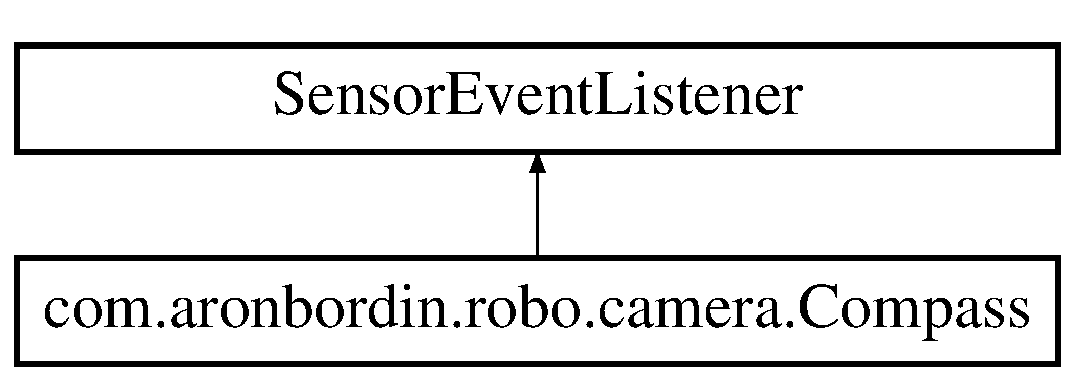
\includegraphics[height=2.000000cm]{dd/d76/classcom_1_1aronbordin_1_1robo_1_1camera_1_1Compass}
\end{center}
\end{figure}
\subsection*{Public Member Functions}
\begin{DoxyCompactItemize}
\item 
\hypertarget{classcom_1_1aronbordin_1_1robo_1_1camera_1_1Compass_ad8fc3c3ff2e46942b4ca3b72522cb69b}{float {\bfseries get\+Direction} ()}\label{classcom_1_1aronbordin_1_1robo_1_1camera_1_1Compass_ad8fc3c3ff2e46942b4ca3b72522cb69b}

\item 
\hypertarget{classcom_1_1aronbordin_1_1robo_1_1camera_1_1Compass_a243c66a814b76eef928a6d66052af458}{void {\bfseries on\+Sensor\+Changed} (Sensor\+Event sensor\+Event)}\label{classcom_1_1aronbordin_1_1robo_1_1camera_1_1Compass_a243c66a814b76eef928a6d66052af458}

\item 
\hypertarget{classcom_1_1aronbordin_1_1robo_1_1camera_1_1Compass_a43a2245d2f010b82efe1c99bddefcb69}{void {\bfseries on\+Accuracy\+Changed} (Sensor sensor, int i)}\label{classcom_1_1aronbordin_1_1robo_1_1camera_1_1Compass_a43a2245d2f010b82efe1c99bddefcb69}

\end{DoxyCompactItemize}
\subsection*{Static Public Member Functions}
\begin{DoxyCompactItemize}
\item 
\hypertarget{classcom_1_1aronbordin_1_1robo_1_1camera_1_1Compass_a2c6b03eadead8f2b81ea95ef062b37db}{static \hyperlink{classcom_1_1aronbordin_1_1robo_1_1camera_1_1Compass}{Compass} {\bfseries get\+Instance} (\hyperlink{classcom_1_1aronbordin_1_1robo_1_1camera_1_1MainActivity}{Main\+Activity} parent)}\label{classcom_1_1aronbordin_1_1robo_1_1camera_1_1Compass_a2c6b03eadead8f2b81ea95ef062b37db}

\end{DoxyCompactItemize}


\subsection{Detailed Description}
\begin{DoxyAuthor}{Author}
Aron Bordin \href{mailto:aron.bordin@gmail.com}{\tt aron.\+bordin@gmail.\+com} Android compass helper 
\end{DoxyAuthor}


The documentation for this class was generated from the following file\+:\begin{DoxyCompactItemize}
\item 
aronbordin/robo/camera/Compass.\+java\end{DoxyCompactItemize}

\hypertarget{classcom_1_1aronbordin_1_1robo_1_1camera_1_1Logger}{\section{com.\+aronbordin.\+robo.\+camera.\+Logger Class Reference}
\label{classcom_1_1aronbordin_1_1robo_1_1camera_1_1Logger}\index{com.\+aronbordin.\+robo.\+camera.\+Logger@{com.\+aronbordin.\+robo.\+camera.\+Logger}}
}
\subsection*{Public Member Functions}
\begin{DoxyCompactItemize}
\item 
void \hyperlink{classcom_1_1aronbordin_1_1robo_1_1camera_1_1Logger_a2eaaf2648c5a95b0ccf221703f4bd97e}{Logar} (String txt)
\item 
void \hyperlink{classcom_1_1aronbordin_1_1robo_1_1camera_1_1Logger_a774dc21499208a63a88b219a76be6e0c}{Logar\+Erro} (String txt)
\end{DoxyCompactItemize}
\subsection*{Protected Attributes}
\begin{DoxyCompactItemize}
\item 
\hypertarget{classcom_1_1aronbordin_1_1robo_1_1camera_1_1Logger_ae1d3ae02ba0a8d6fa91042a5e03bcc4e}{String {\bfseries T\+A\+G} = \char`\"{}Logger\char`\"{}}\label{classcom_1_1aronbordin_1_1robo_1_1camera_1_1Logger_ae1d3ae02ba0a8d6fa91042a5e03bcc4e}

\end{DoxyCompactItemize}


\subsection{Detailed Description}
Created by neo on 08/06/14. \begin{DoxyAuthor}{Author}
Aron Bordin \href{mailto:aron.bordin@gmail.com}{\tt aron.\+bordin@gmail.\+com} Classe responsável por gerenciar os logs do sistema 
\end{DoxyAuthor}


\subsection{Member Function Documentation}
\hypertarget{classcom_1_1aronbordin_1_1robo_1_1camera_1_1Logger_a2eaaf2648c5a95b0ccf221703f4bd97e}{\index{com\+::aronbordin\+::robo\+::camera\+::\+Logger@{com\+::aronbordin\+::robo\+::camera\+::\+Logger}!Logar@{Logar}}
\index{Logar@{Logar}!com\+::aronbordin\+::robo\+::camera\+::\+Logger@{com\+::aronbordin\+::robo\+::camera\+::\+Logger}}
\subsubsection[{Logar}]{\setlength{\rightskip}{0pt plus 5cm}void com.\+aronbordin.\+robo.\+camera.\+Logger.\+Logar (
\begin{DoxyParamCaption}
\item[{String}]{txt}
\end{DoxyParamCaption}
)\hspace{0.3cm}{\ttfamily [inline]}}}\label{classcom_1_1aronbordin_1_1robo_1_1camera_1_1Logger_a2eaaf2648c5a95b0ccf221703f4bd97e}
Loga uma informação para debug 
\begin{DoxyParams}{Parameters}
{\em txt} & texto de debug \\
\hline
\end{DoxyParams}
\hypertarget{classcom_1_1aronbordin_1_1robo_1_1camera_1_1Logger_a774dc21499208a63a88b219a76be6e0c}{\index{com\+::aronbordin\+::robo\+::camera\+::\+Logger@{com\+::aronbordin\+::robo\+::camera\+::\+Logger}!Logar\+Erro@{Logar\+Erro}}
\index{Logar\+Erro@{Logar\+Erro}!com\+::aronbordin\+::robo\+::camera\+::\+Logger@{com\+::aronbordin\+::robo\+::camera\+::\+Logger}}
\subsubsection[{Logar\+Erro}]{\setlength{\rightskip}{0pt plus 5cm}void com.\+aronbordin.\+robo.\+camera.\+Logger.\+Logar\+Erro (
\begin{DoxyParamCaption}
\item[{String}]{txt}
\end{DoxyParamCaption}
)\hspace{0.3cm}{\ttfamily [inline]}}}\label{classcom_1_1aronbordin_1_1robo_1_1camera_1_1Logger_a774dc21499208a63a88b219a76be6e0c}
Loga um erro 
\begin{DoxyParams}{Parameters}
{\em txt} & Erro para logar \\
\hline
\end{DoxyParams}


The documentation for this class was generated from the following file\+:\begin{DoxyCompactItemize}
\item 
aronbordin/robo/camera/Logger.\+java\end{DoxyCompactItemize}

\hypertarget{classcom_1_1aronbordin_1_1robo_1_1camera_1_1MainActivity}{\section{com.\+aronbordin.\+robo.\+camera.\+Main\+Activity Class Reference}
\label{classcom_1_1aronbordin_1_1robo_1_1camera_1_1MainActivity}\index{com.\+aronbordin.\+robo.\+camera.\+Main\+Activity@{com.\+aronbordin.\+robo.\+camera.\+Main\+Activity}}
}
Inheritance diagram for com.\+aronbordin.\+robo.\+camera.\+Main\+Activity\+:\begin{figure}[H]
\begin{center}
\leavevmode
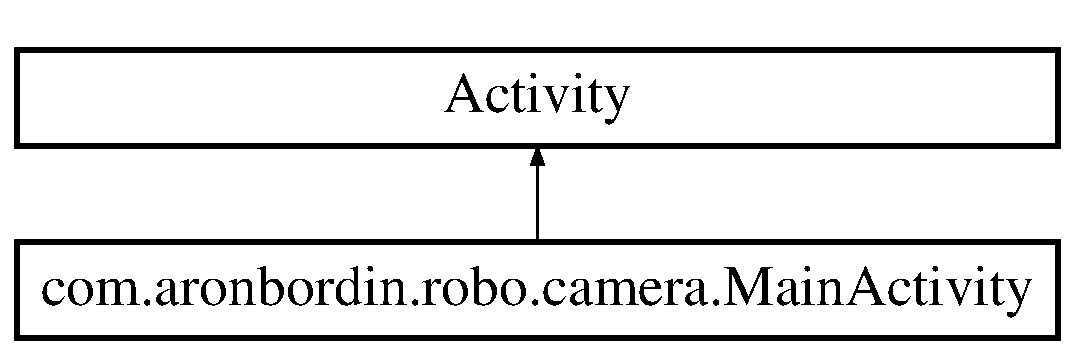
\includegraphics[height=2.000000cm]{dd/da1/classcom_1_1aronbordin_1_1robo_1_1camera_1_1MainActivity}
\end{center}
\end{figure}
\subsection*{Public Member Functions}
\begin{DoxyCompactItemize}
\item 
\hypertarget{classcom_1_1aronbordin_1_1robo_1_1camera_1_1MainActivity_aa93ba91edf8ce75af986c2b514dcb2f5}{void {\bfseries on\+Destroy} ()}\label{classcom_1_1aronbordin_1_1robo_1_1camera_1_1MainActivity_aa93ba91edf8ce75af986c2b514dcb2f5}

\item 
void \hyperlink{classcom_1_1aronbordin_1_1robo_1_1camera_1_1MainActivity_a6cf29e225705388ac8f1314d6c7db928}{iniciar\+Robo} ()
\item 
void \hyperlink{classcom_1_1aronbordin_1_1robo_1_1camera_1_1MainActivity_a05fe1bfdbf4e461a6078cf3353a9da83}{parar\+Robo} ()
\end{DoxyCompactItemize}
\subsection*{Public Attributes}
\begin{DoxyCompactItemize}
\item 
\hypertarget{classcom_1_1aronbordin_1_1robo_1_1camera_1_1MainActivity_a3f9dd2014690d37d73f4e2ec9e0f8f3b}{\hyperlink{classcom_1_1aronbordin_1_1robo_1_1camera_1_1CameraRobo}{Camera\+Robo} {\bfseries m\+Preview}}\label{classcom_1_1aronbordin_1_1robo_1_1camera_1_1MainActivity_a3f9dd2014690d37d73f4e2ec9e0f8f3b}

\item 
\hypertarget{classcom_1_1aronbordin_1_1robo_1_1camera_1_1MainActivity_ab78efbf63f4c132ae0f542615fd7851a}{\hyperlink{classcom_1_1aronbordin_1_1robo_1_1camera_1_1BluetoothRobo}{Bluetooth\+Robo} {\bfseries m\+Bluetooth}}\label{classcom_1_1aronbordin_1_1robo_1_1camera_1_1MainActivity_ab78efbf63f4c132ae0f542615fd7851a}

\item 
\hypertarget{classcom_1_1aronbordin_1_1robo_1_1camera_1_1MainActivity_af03009a4416e8cc5d44a87fa3ae61ca5}{\hyperlink{classcom_1_1aronbordin_1_1robo_1_1camera_1_1Robo}{Robo} {\bfseries m\+Robo}}\label{classcom_1_1aronbordin_1_1robo_1_1camera_1_1MainActivity_af03009a4416e8cc5d44a87fa3ae61ca5}

\item 
\hypertarget{classcom_1_1aronbordin_1_1robo_1_1camera_1_1MainActivity_af596156b326eb6f7d052bcab89f1685d}{\hyperlink{classcom_1_1aronbordin_1_1robo_1_1camera_1_1Logger}{Logger} {\bfseries m\+Logger}}\label{classcom_1_1aronbordin_1_1robo_1_1camera_1_1MainActivity_af596156b326eb6f7d052bcab89f1685d}

\end{DoxyCompactItemize}
\subsection*{Protected Member Functions}
\begin{DoxyCompactItemize}
\item 
void \hyperlink{classcom_1_1aronbordin_1_1robo_1_1camera_1_1MainActivity_a6541ba1e15bcab9d74545566ca5d1ec2}{on\+Create} (Bundle saved\+Instance\+State)
\item 
void \hyperlink{classcom_1_1aronbordin_1_1robo_1_1camera_1_1MainActivity_abe3e630bb05b302a826dad2eccf76bd7}{create\+Camera} ()
\end{DoxyCompactItemize}
\subsection*{Protected Attributes}
\begin{DoxyCompactItemize}
\item 
\hypertarget{classcom_1_1aronbordin_1_1robo_1_1camera_1_1MainActivity_a9e44250adb4b7025eb8d083d7b4bcdf4}{Power\+Manager.\+Wake\+Lock {\bfseries m\+Wake\+Lock}}\label{classcom_1_1aronbordin_1_1robo_1_1camera_1_1MainActivity_a9e44250adb4b7025eb8d083d7b4bcdf4}

\end{DoxyCompactItemize}


\subsection{Detailed Description}
\begin{DoxyAuthor}{Author}
Aron Bordin \href{mailto:aron.bordin@gmail.com}{\tt aron.\+bordin@gmail.\+com} Classe principal, irá iniciar o U\+I e depois a lógica 
\end{DoxyAuthor}


\subsection{Member Function Documentation}
\hypertarget{classcom_1_1aronbordin_1_1robo_1_1camera_1_1MainActivity_abe3e630bb05b302a826dad2eccf76bd7}{\index{com\+::aronbordin\+::robo\+::camera\+::\+Main\+Activity@{com\+::aronbordin\+::robo\+::camera\+::\+Main\+Activity}!create\+Camera@{create\+Camera}}
\index{create\+Camera@{create\+Camera}!com\+::aronbordin\+::robo\+::camera\+::\+Main\+Activity@{com\+::aronbordin\+::robo\+::camera\+::\+Main\+Activity}}
\subsubsection[{create\+Camera}]{\setlength{\rightskip}{0pt plus 5cm}void com.\+aronbordin.\+robo.\+camera.\+Main\+Activity.\+create\+Camera (
\begin{DoxyParamCaption}
{}
\end{DoxyParamCaption}
)\hspace{0.3cm}{\ttfamily [inline]}, {\ttfamily [protected]}}}\label{classcom_1_1aronbordin_1_1robo_1_1camera_1_1MainActivity_abe3e630bb05b302a826dad2eccf76bd7}
Cria o objeto camera, pegando a camera padrão do sistema e rotacionando corretamente \hypertarget{classcom_1_1aronbordin_1_1robo_1_1camera_1_1MainActivity_a6cf29e225705388ac8f1314d6c7db928}{\index{com\+::aronbordin\+::robo\+::camera\+::\+Main\+Activity@{com\+::aronbordin\+::robo\+::camera\+::\+Main\+Activity}!iniciar\+Robo@{iniciar\+Robo}}
\index{iniciar\+Robo@{iniciar\+Robo}!com\+::aronbordin\+::robo\+::camera\+::\+Main\+Activity@{com\+::aronbordin\+::robo\+::camera\+::\+Main\+Activity}}
\subsubsection[{iniciar\+Robo}]{\setlength{\rightskip}{0pt plus 5cm}void com.\+aronbordin.\+robo.\+camera.\+Main\+Activity.\+iniciar\+Robo (
\begin{DoxyParamCaption}
{}
\end{DoxyParamCaption}
)\hspace{0.3cm}{\ttfamily [inline]}}}\label{classcom_1_1aronbordin_1_1robo_1_1camera_1_1MainActivity_a6cf29e225705388ac8f1314d6c7db928}
Método para iniciar a execução do rob$^\wedge$o \hypertarget{classcom_1_1aronbordin_1_1robo_1_1camera_1_1MainActivity_a6541ba1e15bcab9d74545566ca5d1ec2}{\index{com\+::aronbordin\+::robo\+::camera\+::\+Main\+Activity@{com\+::aronbordin\+::robo\+::camera\+::\+Main\+Activity}!on\+Create@{on\+Create}}
\index{on\+Create@{on\+Create}!com\+::aronbordin\+::robo\+::camera\+::\+Main\+Activity@{com\+::aronbordin\+::robo\+::camera\+::\+Main\+Activity}}
\subsubsection[{on\+Create}]{\setlength{\rightskip}{0pt plus 5cm}void com.\+aronbordin.\+robo.\+camera.\+Main\+Activity.\+on\+Create (
\begin{DoxyParamCaption}
\item[{Bundle}]{saved\+Instance\+State}
\end{DoxyParamCaption}
)\hspace{0.3cm}{\ttfamily [inline]}, {\ttfamily [protected]}}}\label{classcom_1_1aronbordin_1_1robo_1_1camera_1_1MainActivity_a6541ba1e15bcab9d74545566ca5d1ec2}
Ao ser criado, inicia todos os objetos do projeto e realiza a conexão Caso tenha algum problema, informa no log $\ast$ 
\begin{DoxyParams}{Parameters}
{\em saved\+Instance\+State} & \\
\hline
\end{DoxyParams}
\hypertarget{classcom_1_1aronbordin_1_1robo_1_1camera_1_1MainActivity_a05fe1bfdbf4e461a6078cf3353a9da83}{\index{com\+::aronbordin\+::robo\+::camera\+::\+Main\+Activity@{com\+::aronbordin\+::robo\+::camera\+::\+Main\+Activity}!parar\+Robo@{parar\+Robo}}
\index{parar\+Robo@{parar\+Robo}!com\+::aronbordin\+::robo\+::camera\+::\+Main\+Activity@{com\+::aronbordin\+::robo\+::camera\+::\+Main\+Activity}}
\subsubsection[{parar\+Robo}]{\setlength{\rightskip}{0pt plus 5cm}void com.\+aronbordin.\+robo.\+camera.\+Main\+Activity.\+parar\+Robo (
\begin{DoxyParamCaption}
{}
\end{DoxyParamCaption}
)\hspace{0.3cm}{\ttfamily [inline]}}}\label{classcom_1_1aronbordin_1_1robo_1_1camera_1_1MainActivity_a05fe1bfdbf4e461a6078cf3353a9da83}
Método para parar o execução do robô 

The documentation for this class was generated from the following file\+:\begin{DoxyCompactItemize}
\item 
aronbordin/robo/camera/Main\+Activity.\+java\end{DoxyCompactItemize}

\hypertarget{classcom_1_1aronbordin_1_1robo_1_1camera_1_1Robo}{\section{com.\+aronbordin.\+robo.\+camera.\+Robo Class Reference}
\label{classcom_1_1aronbordin_1_1robo_1_1camera_1_1Robo}\index{com.\+aronbordin.\+robo.\+camera.\+Robo@{com.\+aronbordin.\+robo.\+camera.\+Robo}}
}
Inheritance diagram for com.\+aronbordin.\+robo.\+camera.\+Robo\+:\begin{figure}[H]
\begin{center}
\leavevmode
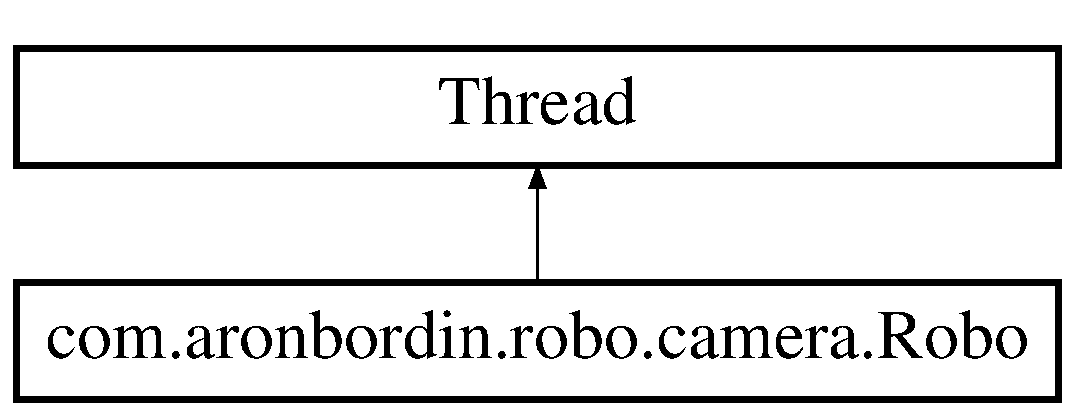
\includegraphics[height=2.000000cm]{df/d6a/classcom_1_1aronbordin_1_1robo_1_1camera_1_1Robo}
\end{center}
\end{figure}
\subsection*{Public Member Functions}
\begin{DoxyCompactItemize}
\item 
\hyperlink{classcom_1_1aronbordin_1_1robo_1_1camera_1_1Robo_a0480d3ff0c17c3acca728036f752c563}{Robo} (\hyperlink{classcom_1_1aronbordin_1_1robo_1_1camera_1_1MainActivity}{Main\+Activity} p)
\item 
void \hyperlink{classcom_1_1aronbordin_1_1robo_1_1camera_1_1Robo_a84b416945e3162ab1b1bb1dea5220339}{Iniciar\+Robo} ()
\item 
void \hyperlink{classcom_1_1aronbordin_1_1robo_1_1camera_1_1Robo_a7fbc061611f1fc6cdd362bedff8d2db4}{Parar\+Robo} ()
\item 
void \hyperlink{classcom_1_1aronbordin_1_1robo_1_1camera_1_1Robo_a04cd1e45ad45e03c773cc4e5ef7dbff7}{run} ()
\item 
\hypertarget{classcom_1_1aronbordin_1_1robo_1_1camera_1_1Robo_a880568348f2029e7451d6c9a087ce473}{void {\bfseries Encruzilhada\+Invertida} ()}\label{classcom_1_1aronbordin_1_1robo_1_1camera_1_1Robo_a880568348f2029e7451d6c9a087ce473}

\item 
\hypertarget{classcom_1_1aronbordin_1_1robo_1_1camera_1_1Robo_a1eeb38dd522233031de91b821e806264}{void {\bfseries Encruzilhada} ()}\label{classcom_1_1aronbordin_1_1robo_1_1camera_1_1Robo_a1eeb38dd522233031de91b821e806264}

\item 
void \hyperlink{classcom_1_1aronbordin_1_1robo_1_1camera_1_1Robo_af4c9ecee2838f22efd53f84b48e14c55}{Desviar} ()
\item 
String \hyperlink{classcom_1_1aronbordin_1_1robo_1_1camera_1_1Robo_af307e730541de825a3017353b06a8667}{pedir\+Valor} (String msg, int id)
\end{DoxyCompactItemize}
\subsection*{Public Attributes}
\begin{DoxyCompactItemize}
\item 
\hypertarget{classcom_1_1aronbordin_1_1robo_1_1camera_1_1Robo_a21717aef50f6816afe957cce92e359d1}{\hyperlink{classcom_1_1aronbordin_1_1robo_1_1camera_1_1Compass}{Compass} {\bfseries m\+Compass}}\label{classcom_1_1aronbordin_1_1robo_1_1camera_1_1Robo_a21717aef50f6816afe957cce92e359d1}

\end{DoxyCompactItemize}
\subsection*{Protected Member Functions}
\begin{DoxyCompactItemize}
\item 
void \hyperlink{classcom_1_1aronbordin_1_1robo_1_1camera_1_1Robo_a390e1e83b708d7c8da9a87d76ac95638}{Loop} ()
\end{DoxyCompactItemize}


\subsection{Detailed Description}
Created by neo on 08/06/14. \begin{DoxyAuthor}{Author}
Aron Bordin \href{mailto:aron.bordin@gmail.com}{\tt aron.\+bordin@gmail.\+com} Classe com toda a lógica do projeto. Irá ler os dados via bluetooth, tomar decisões e movimentar o robô 
\end{DoxyAuthor}


\subsection{Constructor \& Destructor Documentation}
\hypertarget{classcom_1_1aronbordin_1_1robo_1_1camera_1_1Robo_a0480d3ff0c17c3acca728036f752c563}{\index{com\+::aronbordin\+::robo\+::camera\+::\+Robo@{com\+::aronbordin\+::robo\+::camera\+::\+Robo}!Robo@{Robo}}
\index{Robo@{Robo}!com\+::aronbordin\+::robo\+::camera\+::\+Robo@{com\+::aronbordin\+::robo\+::camera\+::\+Robo}}
\subsubsection[{Robo}]{\setlength{\rightskip}{0pt plus 5cm}com.\+aronbordin.\+robo.\+camera.\+Robo.\+Robo (
\begin{DoxyParamCaption}
\item[{{\bf Main\+Activity}}]{p}
\end{DoxyParamCaption}
)\hspace{0.3cm}{\ttfamily [inline]}}}\label{classcom_1_1aronbordin_1_1robo_1_1camera_1_1Robo_a0480d3ff0c17c3acca728036f752c563}
Construtor do objeto. 
\begin{DoxyParams}{Parameters}
{\em p} & parent = \hyperlink{classcom_1_1aronbordin_1_1robo_1_1camera_1_1MainActivity}{Main\+Activity} \\
\hline
\end{DoxyParams}


\subsection{Member Function Documentation}
\hypertarget{classcom_1_1aronbordin_1_1robo_1_1camera_1_1Robo_af4c9ecee2838f22efd53f84b48e14c55}{\index{com\+::aronbordin\+::robo\+::camera\+::\+Robo@{com\+::aronbordin\+::robo\+::camera\+::\+Robo}!Desviar@{Desviar}}
\index{Desviar@{Desviar}!com\+::aronbordin\+::robo\+::camera\+::\+Robo@{com\+::aronbordin\+::robo\+::camera\+::\+Robo}}
\subsubsection[{Desviar}]{\setlength{\rightskip}{0pt plus 5cm}void com.\+aronbordin.\+robo.\+camera.\+Robo.\+Desviar (
\begin{DoxyParamCaption}
{}
\end{DoxyParamCaption}
)\hspace{0.3cm}{\ttfamily [inline]}}}\label{classcom_1_1aronbordin_1_1robo_1_1camera_1_1Robo_af4c9ecee2838f22efd53f84b48e14c55}
Helper para desviar de obstáculo \hypertarget{classcom_1_1aronbordin_1_1robo_1_1camera_1_1Robo_a84b416945e3162ab1b1bb1dea5220339}{\index{com\+::aronbordin\+::robo\+::camera\+::\+Robo@{com\+::aronbordin\+::robo\+::camera\+::\+Robo}!Iniciar\+Robo@{Iniciar\+Robo}}
\index{Iniciar\+Robo@{Iniciar\+Robo}!com\+::aronbordin\+::robo\+::camera\+::\+Robo@{com\+::aronbordin\+::robo\+::camera\+::\+Robo}}
\subsubsection[{Iniciar\+Robo}]{\setlength{\rightskip}{0pt plus 5cm}void com.\+aronbordin.\+robo.\+camera.\+Robo.\+Iniciar\+Robo (
\begin{DoxyParamCaption}
{}
\end{DoxyParamCaption}
)\hspace{0.3cm}{\ttfamily [inline]}}}\label{classcom_1_1aronbordin_1_1robo_1_1camera_1_1Robo_a84b416945e3162ab1b1bb1dea5220339}
Método para iniciar a execução do robô \hypertarget{classcom_1_1aronbordin_1_1robo_1_1camera_1_1Robo_a390e1e83b708d7c8da9a87d76ac95638}{\index{com\+::aronbordin\+::robo\+::camera\+::\+Robo@{com\+::aronbordin\+::robo\+::camera\+::\+Robo}!Loop@{Loop}}
\index{Loop@{Loop}!com\+::aronbordin\+::robo\+::camera\+::\+Robo@{com\+::aronbordin\+::robo\+::camera\+::\+Robo}}
\subsubsection[{Loop}]{\setlength{\rightskip}{0pt plus 5cm}void com.\+aronbordin.\+robo.\+camera.\+Robo.\+Loop (
\begin{DoxyParamCaption}
{}
\end{DoxyParamCaption}
)\hspace{0.3cm}{\ttfamily [inline]}, {\ttfamily [protected]}}}\label{classcom_1_1aronbordin_1_1robo_1_1camera_1_1Robo_a390e1e83b708d7c8da9a87d76ac95638}
Loop principal do robô Executado a cada 20 ms \hypertarget{classcom_1_1aronbordin_1_1robo_1_1camera_1_1Robo_a7fbc061611f1fc6cdd362bedff8d2db4}{\index{com\+::aronbordin\+::robo\+::camera\+::\+Robo@{com\+::aronbordin\+::robo\+::camera\+::\+Robo}!Parar\+Robo@{Parar\+Robo}}
\index{Parar\+Robo@{Parar\+Robo}!com\+::aronbordin\+::robo\+::camera\+::\+Robo@{com\+::aronbordin\+::robo\+::camera\+::\+Robo}}
\subsubsection[{Parar\+Robo}]{\setlength{\rightskip}{0pt plus 5cm}void com.\+aronbordin.\+robo.\+camera.\+Robo.\+Parar\+Robo (
\begin{DoxyParamCaption}
{}
\end{DoxyParamCaption}
)\hspace{0.3cm}{\ttfamily [inline]}}}\label{classcom_1_1aronbordin_1_1robo_1_1camera_1_1Robo_a7fbc061611f1fc6cdd362bedff8d2db4}
Método para parar a execução do robô \hypertarget{classcom_1_1aronbordin_1_1robo_1_1camera_1_1Robo_af307e730541de825a3017353b06a8667}{\index{com\+::aronbordin\+::robo\+::camera\+::\+Robo@{com\+::aronbordin\+::robo\+::camera\+::\+Robo}!pedir\+Valor@{pedir\+Valor}}
\index{pedir\+Valor@{pedir\+Valor}!com\+::aronbordin\+::robo\+::camera\+::\+Robo@{com\+::aronbordin\+::robo\+::camera\+::\+Robo}}
\subsubsection[{pedir\+Valor}]{\setlength{\rightskip}{0pt plus 5cm}String com.\+aronbordin.\+robo.\+camera.\+Robo.\+pedir\+Valor (
\begin{DoxyParamCaption}
\item[{String}]{msg, }
\item[{int}]{id}
\end{DoxyParamCaption}
)\hspace{0.3cm}{\ttfamily [inline]}}}\label{classcom_1_1aronbordin_1_1robo_1_1camera_1_1Robo_af307e730541de825a3017353b06a8667}
Método para enviar uma mensagem ao robô e esperar um retorno 
\begin{DoxyParams}{Parameters}
{\em msg} & Mensagem a ser enviada \\
\hline
{\em id} & I\+D do pedido, para identifiar a mensagem posteriormente \\
\hline
\end{DoxyParams}
\begin{DoxyReturn}{Returns}
String com o valor pedido 
\end{DoxyReturn}
\hypertarget{classcom_1_1aronbordin_1_1robo_1_1camera_1_1Robo_a04cd1e45ad45e03c773cc4e5ef7dbff7}{\index{com\+::aronbordin\+::robo\+::camera\+::\+Robo@{com\+::aronbordin\+::robo\+::camera\+::\+Robo}!run@{run}}
\index{run@{run}!com\+::aronbordin\+::robo\+::camera\+::\+Robo@{com\+::aronbordin\+::robo\+::camera\+::\+Robo}}
\subsubsection[{run}]{\setlength{\rightskip}{0pt plus 5cm}void com.\+aronbordin.\+robo.\+camera.\+Robo.\+run (
\begin{DoxyParamCaption}
{}
\end{DoxyParamCaption}
)\hspace{0.3cm}{\ttfamily [inline]}}}\label{classcom_1_1aronbordin_1_1robo_1_1camera_1_1Robo_a04cd1e45ad45e03c773cc4e5ef7dbff7}
Thread para manter o robô em execução Nunca chame esse método!! Usado internamente para manter o robô em execução 

The documentation for this class was generated from the following file\+:\begin{DoxyCompactItemize}
\item 
aronbordin/robo/camera/Robo.\+java\end{DoxyCompactItemize}

%--- End generated contents ---

% Index
\newpage
\phantomsection
\addcontentsline{toc}{chapter}{Index}
\printindex

\end{document}
